\documentclass{rvcepaper}
\begin{document}

% ---------- HS261TA Principles of Management & Economics (Improvement CIE)
\begin{iempaper}
\paperinfo{shownote=0,date={23\textsuperscript{rd} June 2025},exam={Improvement CIE},maxmarks={10 + 50},sem={VI},prog={UG},duration={30 + 90 Min},
 title={Principles of Management \& Economics},code={HS261TA}}
\iemhead
{\small Note: Answer all the Questions.}\par\vspace{3pt}
\begin{cietable}{M}{BT}{CO}
\qpart{Part -- A}
\q{1.}{Mention the five hierarchical needs proposed by Maslow.}{1}{1}{3}
\q{2.}{State the two factors that form the basis of leadership styles in the Managerial Grid theory.}{1}{1}{3}
\q{3.}{Name the two factors in Herzberg's Two-Factor Theory.}{1}{1}{3}
\q{4.}{An employee feels demotivated because they believe their efforts will not lead to good performance. Which motivation theory explains this situation?}{1}{3}{3}
\q{5.}{An employee compares their effort-reward ratio with a colleague and feels under-rewarded. Which motivation theory does this refer to?}{1}{3}{3}
\q{6.}{A team leader adjusts their leadership style based on the maturity level of team members. Which leadership theory is being applied?}{1}{3}{3}
\q{7.}{Identify the price index used to monitor inflation trends.}{1}{1}{4}
\q{8.}{Name any two main components of Gross Domestic Product (GDP).}{1}{1}{4}
\q{9.}{Which macroeconomic model illustrates the relationship between interest rates and output in goods and money markets?}{1}{2}{4}
\q{10.}{What are the three methods used to calculate GDP?}{1}{1}{4}
\qpart{Part -- B}
\q{1.}{Apply Adams' Equity Theory to explain why an employee may feel demotivated despite consistent high performance and limited rewards. What steps can management take to address this perceived inequity?}{10}{3}{3}
\q{2.}{Explain Hersey and Blanchard's Situational Leadership Theory. How can leaders effectively apply this model to adapt their style based on team members' maturity and competence levels?}{10}{2}{3}
\q{3.}{A manager follows an autocratic approach, assuming that employees inherently dislike work and require constant supervision, leading to low morale. Identify the theory being applied and evaluate how shifting to an alternative perspective could enhance employee motivation.}{10}{3}{3}
\q{4.}{Explain the structure of the IS-LM model and discuss its role in analysing equilibrium in the goods and money markets within macroeconomics.}{10}{2}{4}
\q{5.}{Identify the key components of Gross Domestic Product (GDP). Evaluate the three primary approaches used to measure a country's GDP.}{10}{2}{4}
\end{cietable}
\end{iempaper}

% ---------- IM362IA Supply Chain Management (Improvement CIE)
\begin{iempaper}
\paperinfo{shownote=0,date={23\textsuperscript{rd} June 2025},exam={Improvement CIE},maxmarks={10 + 50},sem={VI},prog={UG},duration={30 + 90 Min},
 title={Supply Chain Management},code={IM362IA}}
\iemhead
{\small Note:}\par\vspace{-1pt}
\hspace*{0.5cm}{\footnotesize 1. \hspace{0.1cm}Answer all the Questions.}\par\vspace{3pt}
\begin{cietable}{M}{BT}{CO}
\qpart{Part -- A}
\q{1.}{The most important operational decision related to transportation in a supply chain is the \blank[2cm] of deliveries.}{1}{L2}{CO2}
\q{2.}{Ignoring inventory costs when making \blank[2cm] decisions can result in choices that worsen the performance of a supply chain.}{1}{L3}{CO2}
\q{3.}{List the two fundamental supply chain decisions involving transportation and inventory cost trade-off.}{1}{L2}{CO1}
\q{4.}{How do third parties increase the supply chain surplus? List any two mechanisms.}{1}{L2}{CO3}
\q{5.}{``Firms must evaluate the risks when they move any function to a third party''. Identify two risks for an automobile manufacturing company.}{2}{L2}{CO3}
\q{6.}{List the processes under CRM.}{2}{L2}{CO4}
\q{7.}{Illustrate the relationship between the three macro processes and the transaction management foundation.}{2}{L2}{CO4}
\qpart{Part -- B}
\q{1}{With the help of a suitable case example elucidate tailored transportation decision made based on size of customer.}{10}{3}{CO2}
\q{2}{Discuss some auction mechanisms that are often used in practice and highlight some of their feature.}{10}{3}{CO3}
\q{3}{Supplier Relationship Management (SRM) includes those processes focused on the interaction between the enterprise and suppliers that are upstream in the supply chain. Evaluate.}{10}{3}{CO3}
\q{4}{Summarize the following managerial actions that increase total supply chain profits and moderate the bullwhip effect.}{10}{2}{CO4}
\q{5}{Explain the significance of continuous replenishment programs and vendor-managed inventories.}{10}{4}{CO4}
\end{cietable}
\end{iempaper}

% ---------- IM363IA Ergonomics (CIE - III)
\begin{iempaper}
\paperinfo{shownote=0,date={24\textsuperscript{th} June 2025},exam={CIE -- III},maxmarks={10 + 50},sem={6\textsuperscript{th}},prog={UG},duration={30 + 90 Min},
 title={ERGONOMICS},code={IM363IA}}
\iemhead
{\small Note:}\par\vspace{-1pt}
\hspace*{0.5cm}{\footnotesize 1. \hspace{0.1cm}Answer all the Questions.}\par\vspace{3pt}
\begin{cietable}{M}{BT}{CO}
\qpart{Part -- A}
\q{1.}{Define static anthropometric data.}{01}{L$_2$}{CO1}
\q{2.}{State one principle of workspace design.}{01}{L$_1$}{CO1}
\q{3.}{What is meant by `reach envelope'?}{01}{L$_2$}{CO2}
\q{4.}{What does the NIOSH lifting equation help assess?}{01}{L$_1$}{CO2}
\q{5.}{State one factor that contributes to low back problems in manual material handling.}{01}{L$_2$}{CO3}
\q{6.}{Name the three stages of the information processing model.}{01}{L$_1$}{CO3}
\q{7.}{Name two interaction styles in Human-Computer Interaction.}{01}{L$_1$}{CO2}
\q{8.}{What does `GOMS' stand for in interface design?}{01}{L$_1$}{CO3}
\q{9.}{In HCI, what is meant by `affordance'?}{01}{L$_2$}{CO3}
\q{10.}{What is meant by `user-task matching' in HCI?}{01}{L$_1$}{CO3}
\qpart{Part -- B}
\q{1.}{Explain the statistical concepts of percentile and variability in human measurements and their relevance in workspace design.}{10}{L$_3$}{CO4}
\q{2.}{Using anthropometric data, design a seated workstation for computer use. Include illustrations of critical dimensions.}{10}{L$_3$}{CO3}
\q{3.}{Discuss the characteristics, limitations, and role of working memory in cognitive tasks.}{10}{L$_4$}{CO4}
\q{4.}{Discuss the concept of time sharing and divided attention. How can multitasking affect task performance in safety-critical environments?}{10}{L$_4$}{CO4}
\q{5.}{Describe the importance of matching interaction styles to users and tasks. Provide examples from mobile applications or web systems.}{10}{L$_4$}{CO3}
\end{cietable}
\end{iempaper}

% ---------- IM365TDA Facilities Planning and Design (Improvement CIE)
\begin{iempaper}
\paperinfo{shownote=0,date={25\textsuperscript{th} June 2025},exam={Improvement CIE},maxmarks={10 + 50},sem={VI},prog={UG},duration={30 + 90 Min},code={IM365TDA},
 title={IM365TDA - FACILITIES PLANNING and DESIGN}}
\begin{center}{\fontsize{12}{14}\selectfont DEPARTMENT OF}\\[3pt]{\bfseries\fontsize{15.5}{18}\selectfont INDUSTRIAL ENGINEERING \& MANAGEMENT}\end{center}\vspace{-3pt}
\noindent\begingroup\renewcommand{\arraystretch}{2.0}\bfseries\fontsize{11.5}{13}\selectfont
\begin{tabular}{|p{6.2cm}|C{5.0cm}|p{5.5cm}|}\hline
 Date \hspace{0.5cm}: \hspace{0.2cm}25\textsuperscript{th} June 2025 & Improvement CIE & Max. Marks \hspace{0.3cm}: \hspace{0.2cm}10 + 50\\\hline
 Semester \hspace{0.1cm}: \hspace{0.2cm}VI & UG & Duration \hspace{0.55cm}: \hspace{0.2cm}30 + 90 Min\\\hline
 \multicolumn{3}{|C{16.7cm}|}{IM365TDA - FACILITIES PLANNING and DESIGN}\\\hline
\end{tabular}\endgroup\par\vspace{4pt}
{\small Note:}\par\vspace{-1pt}
\hspace*{0.5cm}{\footnotesize 1. \hspace{0.1cm}Answer all the Questions.}\par\vspace{3pt}
\ptitle{PART A}
\begin{longtable}{|C{1.05cm}|p{12.2cm}|C{0.95cm}|C{0.95cm}|C{0.95cm}|}
\hline \textbf{Q No.1} & \multicolumn{1}{c|}{\textbf{Questions}} & \textbf{M} & \textbf{BT} & \textbf{CO}\\\hline
\q{1.1}{State one trend in facilities planning aligned with Industry 4.0.}{02}{2}{CO1}
\q{1.2}{What does a pull system in JIT manufacturing imply?}{02}{1}{CO1}
\q{1.3}{Why is reducing Work-In-Process (WIP) important in manufacturing?}{02}{2}{CO1}
\q{1.4}{List the storage operations.}{02}{1}{CO4}
\q{1.5}{Write two principles of order picking.}{02}{2}{CO4}
\end{longtable}
\ptitle{Part --B}
\begin{cietable}{M}{BT}{CO}
\q{1}{Explain the concept of Flexible Manufacturing Systems (FMS). How do they improve production efficiency compared to fixed automation?}{10}{L2}{CO1}
\q{2}{Differentiate between single-stage multi-machine systems and multi-stage systems. Give examples of each.}{10}{L3}{CO3}
\q{3}{Define fixed automation systems. What are their advantages and limitations in mass production environments?}{10}{L2}{CO2}
\q{4}{Sketch and explain the functions in the warehouse.}{10}{L3}{CO4}
\q{5}{Enumerate and elaborate shipping principles.}{10}{L1}{CO4}
\end{cietable}
\end{iempaper}

% ---------- IM364TA Human Resource Management & Analytics (CIE - III)
\begin{iempaper}
\paperinfo{shownote=0,date={24\textsuperscript{th} June 2025},exam={CIE -- III},maxmarks={10 + 50},sem={VI},prog={UG},duration={30 + 90 Min},
 title={Human Resource Management \& Analytics - IM364TA},code={IM364TA}}
\begin{center}{\fontsize{12}{14}\selectfont DEPARTMENT OF}\\[3pt]{\bfseries\fontsize{15.5}{18}\selectfont INDUSTRIAL ENGINEERING \& MANAGEMENT}\end{center}\vspace{-3pt}
\noindent\begingroup\renewcommand{\arraystretch}{2.0}\bfseries\fontsize{11.5}{13}\selectfont
\begin{tabular}{|p{6.2cm}|C{5.0cm}|p{5.5cm}|}\hline
 Date \hspace{0.5cm}: \hspace{0.2cm}24\textsuperscript{th} June 2025 & CIE -- III & Max. Marks \hspace{0.3cm}: \hspace{0.2cm}10 + 50\\\hline
 Semester \hspace{0.1cm}: \hspace{0.2cm}VI & UG & Duration \hspace{0.55cm}: \hspace{0.2cm}30 + 90 Min\\\hline
 \multicolumn{3}{|C{16.7cm}|}{Human Resource Management \& Analytics - IM364TA}\\\hline
\end{tabular}\endgroup\par\vspace{4pt}
{\small Note:}\par\vspace{-1pt}
\hspace*{0.5cm}{\footnotesize 1. \hspace{0.1cm}Answer all the Questions.}\par\vspace{3pt}
\begin{cietable}{M}{BT}{CO}
\qpart{Part -- A}
\q{1.}{What is an HR Scorecard?}{02}{L1}{CO4}
\q{2.}{What is the role of regression analysis in HR analytics?}{02}{L2}{CO4}
\q{3.}{Name any two phases in the HR predictive modelling process.}{02}{L2}{CO4}
\q{4.}{Name any two software tools used for HR predictive analytics.}{02}{L1}{CO4}
\q{5.}{What is sentiment analysis and how is it useful in HR analytics?}{02}{L2}{CO4}
\qpart{Part -- B}
\q{1.}{Explain how an HR scorecard is developed in an organization. Design a scorecard for talent management function.}{10}{L2}{CO4}
\q{2.}{You want to design an HR dashboard on performance management issues for the sales force of your organization. Based on your identified list of issues, choose at least two important issues and design an illustrative dashboard.}{10}{L3}{CO4}
\q{3.}{As an HR manager, you're tasked with designing a data collection process for a training needs analysis. What data sources and methods will you use, and how will you ensure data accuracy?}{10}{L3}{CO4}
\q{4.}{You are presenting a monthly HR report to the executive team. Choose three key metrics to include and explain how each one contributes to strategic business decisions.}{10}{L2}{CO4}
\q{5.}{What are the key tools and techniques used in predictive HR analytics? Illustrate with examples how decision trees or logistic regression can solve HR problems.}{10}{L2}{CO4}
\end{cietable}
\stars{----*****----}
\end{iempaper}

% ---------- IM266TEQ Elements of Financial Management (CIE - III)
\begin{iempaperB}
\paperinfo{hdr=2,ayear={2024-2025 (EVEN Sem)},date={25\textsuperscript{th} June 2025},code={IM266TEQ},sem={VII Semester},exam={CIE -- III},maxmarks={10 + 50},duration={120 Mins},
 title={ELEMENTS OF FINANCIAL MANAGEMENT},shownote=0}
\iemheadB
{\small Note:}\par\vspace{-1pt}
\hspace*{0.5cm}{\footnotesize 1. \hspace{0.1cm}Answer all the Questions.}\par
\hspace*{0.5cm}{\footnotesize 2. \hspace{0.1cm}Avoid verbose answers and answer specifically and to the point.}\par\vspace{3pt}
\ptitle{PART -- A}
\begin{xtable}{Questions}
\q{1}{what are the key differences between debt and equity?}{02}{L$_1$}{CO1}
\q{2}{How should a business person use debentures as an instrument as opposed to venture capital?}{02}{L$_2$}{CO1}
\q{3}{List any three sources of internal accruals}{02}{L$_1$}{CO1}
\q{4}{Mention two disadvantages of raising funds through an IPO.}{02}{L$_1$}{CO1}
\q{5}{Who issues Government securities market and for what purpose?}{02}{L$_1$}{CO1}
\end{xtable}
\ptitle{PART -- B}
\begin{xtable}{Questions}
\q{1.}{What is preference capital? Explain its key features in brief.}{10}{L2}{CO1}
\q{2.}{Write short notes on
\begin{romi}\item[i.] Initial Public offer\item[ii.] Debentures\item[iii.] Term Loans\item[iv.] Investment Banking\end{romi}}{10}{L3}{CO1}
\q{3}{Differentiate between the primary market and secondary market with examples.}{10}{L2}{CO2}
\q{4.}{What are the key features of venture capital. How do they differ from traditional financing methods.}{10}{L2}{CO3}
\q{5.}{Differentiate between Operating Cycle and Cash Cycle. Explain their significance in working capital management with suitable examples.}{10}{L3}{CO1}
\end{xtable}
\end{iempaperB}

% ---------- HS266TEW Applied Psychology for Engineers (Improvement Test)
\begin{iempaper}
\paperinfo{shownote=0,date={25.06.2025},exam={CIE-- Improvement Test},maxmarks={10 + 50},sem={VI},prog={UG- Institutional Elective},duration={30 + 90 Min},
 title={Applied Psychology for Engineers},code={HS266TEW}}
\begin{center}{\fontsize{12}{14}\selectfont DEPARTMENT OF}\\[3pt]{\bfseries\fontsize{15.5}{18}\selectfont HUMANITIES AND SOCIAL SCIENCES}\end{center}\vspace{-3pt}
\noindent\begingroup\renewcommand{\arraystretch}{2.0}\bfseries\fontsize{11.5}{13}\selectfont
\begin{tabular}{|p{6.2cm}|C{5.0cm}|p{5.5cm}|}\hline
 Date \hspace{0.5cm}: \hspace{0.2cm}25.06.2025 & CIE-- Improvement Test & Max. Marks \hspace{0.3cm}: \hspace{0.2cm}10 + 50\\\hline
 Semester \hspace{0.1cm}: \hspace{0.2cm}VI & UG- Institutional Elective & Duration \hspace{0.55cm}: \hspace{0.2cm}30 + 90 Min\\\hline
 \multicolumn{2}{|p{11.2cm}|}{Course Title: Applied Psychology for Engineers} & Course Code \hspace{0.1cm}: \hspace{0.2cm}HS266TEW\\\hline
\end{tabular}\endgroup\par\vspace{4pt}
{\small Note:}\par\vspace{-1pt}
\hspace*{0.5cm}{\footnotesize Answer all the Questions}\par\vspace{3pt}
\begin{cietable}{M}{BT}{CO}
\qpart{Part -- A}
\q{1}{Every time Riya touches a hot utensil, she quickly pulls her hand back. Over time, she learns to avoid touching them altogether. Which type of learning is illustrated in Riya's case?}{2}{L1}{CO1}
\q{2}{Seema was unable to switch on her new blender as it had no visible button. After examining it for a while, she suddenly realized that it turned on when the lid was locked in place. Identify the type of learning involved and mention two strategies used.}{2}{L2}{CO2}
\q{3}{Mention the role of psychologists in the IT environment.}{2}{L2}{CO3}
\q{4}{What are the information technology tools that are used in distance learning?}{2}{L2}{CO4}
\q{5}{Nina has been feeling constantly stressed due to academic pressure and finds it hard to manage her emotions. She approaches the college counsellor for help. What type of psychological counselling does Nina require?}{2}{L1}{CO3}
\qpart{Part -- B}
\q{1}{Every time Meena took her dog out, she used a bell to signal feeding time. Soon, the dog began salivating just at the sound of the bell, even when no food was present. Apply the concept of classical conditioning to explain the dog's behavior. Identify the UCS, UCR, CS, and CR, and describe any two principles of classical conditioning.}{10}{L2}{CO1}
\q{2}{An employee was scolded by his manager each time he arrived late to work. Eventually, he started coming on time to avoid being scolded. Using the concept of Operant Conditioning, explain Rahul's change in behavior.}{10}{L2}{CO2}
\q{3}{Ravi recently joined a new office and felt unsure about how to interact during team meetings. Over the next few weeks, he carefully observed his senior colleagues---how they presented ideas, maintained body language, and responded to feedback. Gradually, Ravi began to adopt similar behaviors and felt more confident participating in discussions. Based on the above case, explain how observational learning operates in social and professional settings.}{10}{L3}{CO2}
\q{4}{An IT company is expanding its workforce and wants to hire psychological professionals to support employee well-being and improve workplace mental health. The HR manager is responsible for selecting and training the right candidates for this role. Explain the steps involved in the selection and training of psychological professionals to work in an organization, using the case above as context.}{10}{L2}{CO2}
\q{5}{What is the basic need for Counselling? Identify and explain the type of counseling the case below is referring to.\newline
An Engineering student has fallen ill twice before his Mathematics tests. He slowly developed anxiety that his health would fail, and so strongly believes and has a fear that something bad would happen before his exams, and refuses to attend the exams.}{10}{L4}{CO2}
\end{cietable}
\end{iempaper}

% ---------- EC266TEH Human Machine Interface (Improvement Test)
\begin{xpaper}
\paperinfo{deptline={Department of Electronics and Communication Engineering},date={25.6.2025},exam={Improvement Test},maxmarks={50},sem={VI},prog={UG},duration={$1\frac{1}{2}$ Hrs $+\frac{1}{2}$ Hrs},
 title={Human Machine Interface},code={EC266TEH}}
\xhead
\begin{xtable}{Questions}
\q{1.a.}{Summarize the different types of HMI Data Analytics.}{4}{1}{1}
\q{1.b.}{What is HMI Profiling? Discuss the different types profiling parameters with an example.}{6}{2}{1}
\q{2.a.}{Discuss different types of haptic feedback and their applications.}{4}{2}{2}
\q{2.b.}{Illustrate the Bosch Graphic Test System with a neat block diagram. Also discuss the features of the same.}{6}{2}{1}
\q{3.a.}{List the different types of HMI Debugging. Discuss the different steps followed for Debugging methods.}{5}{2}{2}
\q{3.b.}{Discuss the different types of challenges in HMI testing.}{5}{2}{2}
\q{4.a.}{Write HTML code to create a \textbf{web-based dashboard} that displays:
\begin{bul}\item Machine ID\item Temperature (in \textdegree C)\item Pressure (in Bar)\item Motor Status (Running/Stopped)\end{bul}}{4}{2}{1}
\q{4.b.}{With a neat block diagram, explain gesture based HMI for Industrial Applications.}{5}{3}{2}
\q{5.a.}{Explain the system architecture used in haptic technology with a neat block diagram.}{6}{3}{3}
\q{5.b.}{Discuss the integration of PLC, motion control, and HMI within the TwinCAT environment.}{5}{1}{1}
\end{xtable}
\par\vspace{6pt}
\begin{xtable}{Improvement - Quiz}
\q{1.}{TwinCAT supports \blank[1.8cm] standard programming languages.}{1}{1}{1}
\q{2.}{\blank[1.8cm] is the correct CSS syntax to change the background color of an element to blue.}{1}{2}{1}
\q{3.}{\blank[1.8cm] is the correct HTML for creating a hyperlink.}{1}{2}{2}
\q{4.}{Which testing capabilities are included in the Bosch Graphics Test System?}{1}{1}{1}
\q{5.}{\blank[1.8cm] diagnostic tool is typically used to verify IP-level connectivity between an HMI and a controller.}{1}{1}{1}
\q{6.}{\blank[1.8cm] Unicode encoding is widely used to support multiple languages in HMI software.}{1}{2}{1}
\q{7.}{Haptics feedback can be realized in the form of Force, \blank[1.8cm], and \blank[1.8cm].}{1}{2}{3}
\q{8.}{Unity is a cross-platform game engine developed by \blank[1.8cm].}{1}{1}{1}
\q{9.}{\blank[1.8cm] metric is often measured during HMI profiling to assess \ldots}{1}{1}{1}
\end{xtable}
\end{xpaper}

% ---------- CM266TEG Advanced Energy Storage for E-Mobility (Quiz)
\begin{xpaper}
\paperinfo{deptline={Department of Chemistry},date={25-06-2025},exam={Quiz},maxmarks={10},sem={6},prog={UG},duration={30 min},
 title={ADVANCED ENERGY STORAGE FOR E-MOBILITY},code={CM266TEG}}
\xhead
\begin{longtable}{|C{1.05cm}|p{12.2cm}|C{0.95cm}|C{0.95cm}|C{0.95cm}|}
\hline \textbf{SI NO} & \multicolumn{1}{c|}{\textbf{Questions}} & \textbf{M} & \textbf{BT} & \textbf{CO}\\\hline
\q{1}{What is regenerative braking?}{1}{1}{1}
\q{2}{Give an example for reserve battery.}{1}{2}{1}
\q{3}{Identify the effect of molar mass on the capacity of the battery.}{1}{2}{2}
\q{4}{Name a lithium based primary battery.}{1}{3}{1}
\q{5}{Which type of electrolyte is used in methanol fuel cell?}{1}{1}{1}
\q{6}{Pseudo capacitors are superior than that of EDLC type super capacitor. Justify}{1}{5}{4}
\q{7}{Solar cell hybrid vehicles are not a good alternative for gasoline vehicles. Justify.}{1}{5}{4}
\q{8}{Give general representation of hydrogen oxygen fuel cells.}{1}{3}{2}
\q{9}{In fuel cell, design of porous electrode along with catalyst is challenging. Justify.}{1}{5}{4}
\q{10}{List any two major advantage of supercapacitor hybrid vehicles.}{1}{2}{2}
\end{longtable}
\end{xpaper}

% ---------- CM266TEG Advanced Energy Storage for E-Mobility (Improvement Test)
\begin{xpaper}
\paperinfo{deptline={Department of Chemistry},date={25-06-2025},exam={Improvement Test},maxmarks={50},sem={6},prog={UG},duration={$1\frac{1}{2}$ Hrs},
 title={ADVANCED ENERGY STORAGE FOR E-MOBILITY},code={CM266TEG}}
\xhead
\begin{longtable}{|C{1.05cm}|p{12.2cm}|C{0.95cm}|C{0.95cm}|C{0.95cm}|}
\hline \textbf{S No} & \multicolumn{1}{c|}{\textbf{Questions}} & \textbf{M} & \textbf{BT} & \textbf{CO}\\\hline
\q{1}{Discuss the salient feature of the following along with neat labelled diagram/flowchart.\newline i)Plug in hybrid vehicles\hspace{1cm}ii) Fuel cell hybrid vehicles}{10}{3}{3}
\q{2}{Analyse any five battery characteristics with respect to advanced battery used in e mobility.}{10}{2}{1}
\q{3}{Outline the construction and working mechanism of Pseudo supercapacitor and EDLC. Along with neat labelled diagram how they help in sustainable transport in super capacitor vehicles?}{10}{4}{2}
\q{4}{By applying the knowledge of semiconductors, Illustrate construction and working of amorphous silicon solar cell along with neat labelled diagram. How these solar cells are used to construct of solar cell hybrid vehicles? Explain the working of it with flow chart.}{10}{3}{2}
\q{5}{Methanol based fuel cell vehicles are good alternative to gasoline vehicles. Justify. Explain the construction and working of methanol oxygen fuel cell along with their advantages and limitations.}{10}{2}{2}
\end{longtable}
\end{xpaper}

% ---------- CV266TEE Intelligent Transportation System (Improvement CIE)
\begin{xpaper}
\paperinfo{deptline={Department of Civil Engineering},date={25-06-2025},exam={Improvement CIE},maxmarks={60},sem={VI},prog={UG},duration={2 Hrs},
 title={Intelligent Transportation System},code={CV266TEE}}
\xhead
\ptitle{Quiz}
\begin{longtable}{|C{1.05cm}|p{12.2cm}|C{0.95cm}|C{0.95cm}|C{0.95cm}|}
\hline \textbf{S No} & \multicolumn{1}{c|}{\textbf{Questions}} & \textbf{M} & \textbf{BT} & \textbf{CO}\\\hline
\q{1.}{Mention any two advanced traffic management measures used in urban areas.}{2}{2}{3}
\q{2.}{List any two objectives of a Traffic Management System}{2}{1}{4}
\q{3.}{List two key technologies used in Advanced Traveller Information Systems (ATIS).}{2}{1}{3}
\q{4.}{Summarize the development stages of a Traffic Management System in brief.}{2}{2}{3}
\q{5.}{State any two benefits of implementing Advance Vehicle Control Systems in modern vehicles.}{2}{2}{4}
\end{longtable}
\par\vspace{6pt}
\begin{longtable}{|C{1.05cm}|p{12.2cm}|C{0.95cm}|C{0.95cm}|C{0.95cm}|}
\hline \textbf{S No} & \multicolumn{1}{c|}{\textbf{Questions}} & \textbf{M} & \textbf{BT} & \textbf{CO}\\\hline
\q{1.}{Discuss the objectives and strategies involved in the development of an efficient Traffic Management System in smart cities.}{10}{3}{3}
\q{2.}{Design a functional layout of a Traffic Management Centre for a tier-2 city and explain the systems integrated within it.}{10}{5}{3}
\q{3.}{Design an outline for the development of a city-wide ITS-based Traffic Management Centre integrating ATMS, ATIS, and APTS.}{10}{5}{4}
\q{4.}{Evaluate the role of ITS in enhancing road safety and traffic efficiency in metropolitan cities.}{10}{4}{3}
\q{5.}{Analyze the technical and operational challenges faced in implementing AVCS in developing countries and propose feasible solutions.}{10}{3}{4}
\end{longtable}
\end{xpaper}

% ---------- CS266TED Robotic Process Automation (Test - 3)
\begin{xpaper}
\paperinfo{deptline={Department of Computer Science and Engineering},date={June 2025},exam={Test - 3},maxmarks={60},sem={VI},prog={UG},duration={2 Hrs},
 title={ROBOTIC PROCESS AUTOMATION},code={CS266TED}}
\xhead
\begin{longtable}{|C{1.05cm}|p{12.2cm}|C{0.95cm}|C{0.95cm}|C{0.95cm}|}
\hline \textbf{Sln} & \multicolumn{1}{c|}{\textbf{PART A Questions}} & \textbf{M} & \textbf{BT} & \textbf{CO}\\\hline
\q{1.}{Name any two UiPath activities used for email automation.}{02}{2}{3}
\q{2.}{A \blank[2cm] in Orchestrator is used to automatically start jobs at specific times or events.}{01}{2}{3}
\q{3.}{In email automation, attachments can be saved using the \blank[2cm] property of the email message object.}{01}{1}{3}
\q{4.}{What is the key difference between the `Breakpoint' and `Log Message' activities, and how do they complement each other during debugging?}{02}{1}{4}
\q{5.}{Mention two core technologies commonly used in hyperautomation.}{02}{2}{4}
\q{6.}{A \blank[2cm] is a debugging tool used to pause execution at a specific point to examine variables and flow.}{01}{2}{3}
\q{7.}{Robots are connected to Orchestrator using a Machine Key and \blank[2cm].}{01}{1}{3}
\end{longtable}
\ptitle{PART B Questions}
\begin{longtable}{|C{1.05cm}|p{12.2cm}|C{0.95cm}|C{0.95cm}|C{0.95cm}|}
\hline \q{1. a}{Explain the role of email protocols in email automation. How are these protocols used in UiPath? Discuss various associated activities in UiPath.}{10}{2}{3}
\q{2. a}{Differentiate between system exceptions and business exceptions in UiPath. Provide examples}{06}{2}{3}
\q{b}{What are the key debugging tools available in UiPath Studio? How do they assist in error resolution?}{04}{3}{3}
\q{3. a}{Explain the structure and function of Try-Catch activity in UiPath. How does it help in managing exceptions?}{04}{3}{3}
\q{b}{What is UiPath Orchestrator? Describe its main functionalities in the context of deploying and managing bots}{06}{2}{3}
\q{4. a}{Discuss the role of queues, assets, and logs in UiPath Orchestrator. How do they support bot management and execution?}{06}{3}{4}
\q{b}{Define hyperautomation and discuss its key components.}{04}{2}{4}
\q{5. a}{List and explain the key phases of hyperautomation. Illustrate any two real-world use cases of hyperautomation}{05}{3}{4}
\q{b}{Explain the concept of Hyperautomation-as-a-Service (HaaS). What are its benefits for small and medium-sized enterprises (SMEs)?}{05}{2}{4}
\end{longtable}
\cotable{\textbf{Course Outcomes}}{CO1 & Understand RPA principles, its features and applications\\\hline CO2 & Demonstrate proficiency in handling variables and decision making inside a workflow and data manipulation techniques.\\\hline CO3 & Gain insights into recording, email automation and exception handling and orchestrator\\\hline CO4 & Analyze the trends in automation and choose business strategy to design a real world automation workflow.}
\btfoot{|l|*{6}{C{1.1cm}|}*{5}{C{1.2cm}|}}{\hline BT \& CO Marks & L1 & L2 & L3 & L4 & L5 & L6 & CO1 & CO2 & CO3 & CO4 & CO5\\\hline & 4 & 37 & 19 & -- & -- & -- & -- & -- & 36 & 24 & --\\\hline}
\end{xpaper}

% ---------- MA266TEV Mathematics of Quantum Computing (CIE 3)
\begin{xpaper}
\paperinfo{deptline={Department of Mathematics},date={25-06-2025},exam={CIE 3},maxmarks={10+50},sem={VI},prog={UG},duration={2 Hrs (2PM - 4PM)},
 title={Mathematics of Quantum Computing},code={MA266TEV}}
\xhead
\begin{longtable}{|C{1.05cm}|p{12.2cm}|C{0.95cm}|C{0.95cm}|C{0.95cm}|}
\hline \textbf{S No} & \multicolumn{1}{c|}{\textbf{Quiz}} & \textbf{M} & \textbf{BT} & \textbf{CO}\\\hline
\q{1}{If the estimated phase in Quantum Phase Estimation algorithm is $\theta=2\pi\left(\frac{3}{8}\right)$, what will be the output of the top register in binary?}{2}{2}{2}
\q{2}{In Shor's algorithm, what is the classical problem reduced to after finding the period $r$ of $a^x$ mod $N$?}{2}{1}{1}
\q{3}{What is the effect of the Grover diffusion operator on the state vector?}{2}{2}{3}
\q{4}{Describe in one sentence how Quantum Phase Estimation is used in both Shor's and HHL algorithms.}{2}{3}{3}
\q{5}{What quantum algorithm is used as a subroutine in Shor's algorithm to find the period of a function?}{1}{2}{2}
\q{6}{In the controlled rotation step of the HHL algorithm, what is encoded into the amplitude of the ancilla qubit?}{1}{1}{1}
\end{longtable}
\begin{longtable}{|C{1.05cm}|p{12.2cm}|C{0.95cm}|C{0.95cm}|C{0.95cm}|}
\hline \textbf{S No} & \multicolumn{1}{c|}{\textbf{Test}} & \textbf{M} & \textbf{BT} & \textbf{CO}\\\hline
\q{1}{State the problem that the Quantum Phase Estimation algorithm is designed to solve. Describe the complete quantum circuit used for QPE, including the role of each register and gate explaining step by step how the algorithm estimates the phase.}{10}{2}{2}
\q{2}{What is the significance of Shor's algorithm in cryptography? Explain how the period $r$ is found out in this algorithm, thereby leading to determining the factorization of the given number $N$.}{10}{3}{3}
\q{3}{Outline the working of Grover's search algorithm explaining the reflections involved. Also analyse the number of iterations involved.}{10}{3}{4}
\q{4}{What are the key assumptions required for the efficiency of HHL algorithm? How does the algorithm solve the quantum version of the problem $A\vec{x}=\vec{b}$? Outline the high-level steps.}{10}{4}{3}
\q{5}{For a 2 qubit search space with one marked state $|11\rangle$, compute the state after one iteration of the Grover operator starting from the uniform superposition state, and verify the probability of measuring the marked state.}{10}{4}{4}
\end{longtable}
\end{xpaper}

% ---------- MA266TEU Mathematical Modelling (Improvement CIE)
\begin{xpaper}
\paperinfo{deptline={Department of Mathematics},date={25/06/2025},exam={Improvement CIE},maxmarks={100},sem={VI},prog={UG},duration={2 Hrs. (2pm-4pm)},
 title={Mathematical Modelling},code={MA266TEU}}
\xhead
\ptitle{Quiz}
\begin{longtable}{|C{1.05cm}|p{12.2cm}|C{0.95cm}|C{0.95cm}|C{0.95cm}|}
\hline \textbf{SL. No} & \multicolumn{1}{c|}{\textbf{Questions}} & \textbf{M} & \textbf{BTL} & \textbf{CO}\\\hline
\q{1}{Is the given graph $G$ balanced? Find the degree of balance of $G$:
\par\vspace{4pt}\centerline{\begin{tikzpicture}[x=1cm,y=1cm,>={Stealth[length=2mm]},font=\small]
\coordinate (T) at (0,2.8); \coordinate (R1) at (1.5,2.1); \coordinate (R2) at (2.0,0.4); \coordinate (L) at (-0.8,0.9); \coordinate (B) at (0.4,-1.0);
\foreach \p in {T,R1,R2,L,B} {\fill (\p) circle (1.2pt);}
\draw[->] (L) -- node[left,pos=0.5] {$+$} (T);
\draw[->] (R1) -- node[above,pos=0.5] {$-$} (T);
\draw[->] (R2) -- node[right,pos=0.5] {$+$} (R1);
\draw[->] (T) -- node[left,pos=0.45] {$-$} (R2);
\draw[->] (R2) -- node[above,pos=0.5] {$-$} (L);
\draw[->] (L) -- node[left,pos=0.5] {$+$} (B);
\draw[->] (B) -- node[right,pos=0.5] {$+$} (R2);
\node[left] at (-1.5,1.2) {$G$:};
\end{tikzpicture}}}{2}{2}{2}
\q{2}{Draw the complete graph $K_{3,4}$.}{2}{1}{1}
\q{3}{Model a real life scenario using a digraph.}{2}{1}{1}
\q{4}{Define bipartite graph with an example.}{2}{3}{2}
\q{5}{The chromatic number of the following graph $H$.
\par\vspace{4pt}\centerline{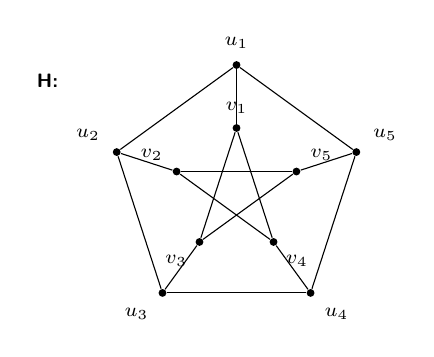
\begin{tikzpicture}[x=1cm,y=1cm,font=\scriptsize,vtx/.style={circle,fill,inner sep=1pt}]
\foreach \i in {1,...,5} {\node[vtx,label={[label distance=1pt]{90+72*(\i-1)}:$u_\i$}] (u\i) at ({90+72*(\i-1)}:1.6) {}; \node[vtx,label={[label distance=0pt]{90+72*(\i-1)}:$v_\i$}] (v\i) at ({90+72*(\i-1)}:0.8) {};}
\foreach \i/\j in {1/2,2/3,3/4,4/5,5/1} {\draw (u\i) -- (u\j);}
\foreach \i in {1,...,5} {\draw (u\i) -- (v\i);}
\foreach \i/\j in {1/3,3/5,5/2,2/4,4/1} {\draw (v\i) -- (v\j);}
\node at (-2.4,1.4) {\sffamily\bfseries H:};
\end{tikzpicture}}}{2}{3}{3}
\end{longtable}
\par\vspace{6pt}
\begin{longtable}{|C{1.05cm}|p{12.2cm}|C{0.95cm}|C{0.95cm}|C{0.95cm}|}
\hline \textbf{SL. No} & \multicolumn{1}{c|}{\textbf{Test}} & \textbf{M} & \textbf{BTL} & \textbf{CO}\\\hline
\q{1.}{Define the Harary measure of status. Find the Harary measure of each individual in the organizational graph shown in the figure below.
\par\vspace{4pt}\centerline{\begin{tikzpicture}[x=1cm,y=1cm,>={Stealth[length=2mm]},font=\scriptsize,nd/.style={draw,rounded corners=2pt,inner sep=2pt}]
\node[nd] (lion) at (-1.6,1.9) {Lion}; \node[nd] (jac) at (0.4,1.9) {Jackal}; \node[nd] (goat) at (2.2,1.1) {Goat};
\node[nd] (eagle) at (-2.4,0.3) {Eagle}; \node[nd] (cat) at (-0.2,0.5) {Wild cat}; \node[nd] (plant) at (2.2,-0.8) {Green Plant};
\node[nd] (owl) at (-1.2,-1.0) {Owl}; \node[nd] (rab) at (0.8,-0.6) {Rabbit}; \node[nd] (snake) at (-2.4,-1.8) {Snake}; \node[nd] (mouse) at (0.2,-1.8) {Mouse};
\draw[->,dashed] (jac) -- (lion); \draw[->,dashed] (goat) -- (lion); \draw[->,dashed] (goat) -- (jac); \draw[->,dashed] (cat) -- (lion);
\draw[->,dashed] (plant) -- (goat); \draw[->,dashed] (plant) -- (rab); \draw[->,dashed] (plant) -- (mouse);
\draw[->,dashed] (rab) -- (cat); \draw[->,dashed] (mouse) -- (owl); \draw[->,dashed] (mouse) -- (snake); \draw[->,dashed] (snake) -- (eagle); \draw[->,dashed] (owl) -- (cat); \draw[->,dashed] (eagle) -- (lion);
\end{tikzpicture}}}{10}{1}{1}
\q{2.}{The Mathematics department of a certain college plans to schedule the classes Graph Theory (GT), Statistics (S), Linear Algebra (LA), Advanced Calculus(AC), Geometry (G) and Modern Algebra (MA) this summer. Ten students given below have indicated the course they plan to take. With this information, use graph theory to determine the minimum number of time periods needed to offer these courses so that every two classes having student in common are taught at different time periods during the day. Of course, two classes having no students in common can be taught during the same period.
\par\vspace{4pt}\noindent Anden: LA,S,\ \ Brynn: MA,LA,G,\ \ Chase: MA, G,LA,\ \ Denise: G, LA, AC\par\vspace{3pt}
\noindent Everett: AC, LA, S,\ \ Francois: G,AC,\ \ Greg: GT, MA, LA\ \ Harper: LA, GT,S\par\vspace{3pt}
\noindent Irene: AC, S, LA\ \ \ \ Jennie: GT, S}{10}{2}{3}
\q{3.}{At the end of the school day, all the students plan on driving from school (Vertex A) to the concert (Vertex Z). The edges in the graph below represent one-way roads, and the weights of each edge represents the number of vehicles (in hundreds) that particular road can handle in one hour. What is the greatest number of vehicles that can get from school.
\par\vspace{4pt}\centerline{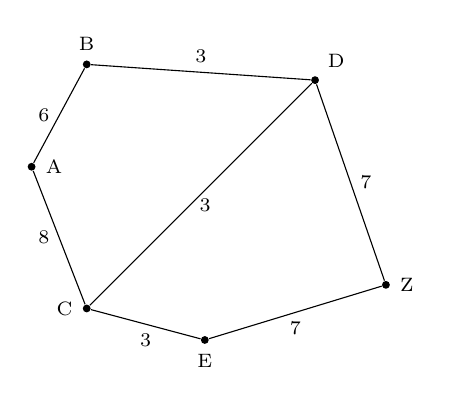
\begin{tikzpicture}[x=1cm,y=1cm,font=\scriptsize,vtx/.style={circle,fill,inner sep=1pt}]
\node[vtx,label={above:B}] (B) at (0,2.2) {}; \node[vtx,label={above right:D}] (D) at (2.9,2.0) {}; \node[vtx,label={right:A}] (A) at (-0.7,0.9) {}; \node[vtx,label={left:C}] (C) at (0.0,-0.9) {}; \node[vtx,label={below:E}] (E) at (1.5,-1.3) {}; \node[vtx,label={right:Z}] (Z) at (3.8,-0.6) {};
\draw (B) -- node[above] {3} (D); \draw (B) -- node[left] {6} (A); \draw (A) -- node[left] {8} (C); \draw (D) -- node[right] {7} (Z); \draw (D) -- node[right,pos=0.55] {3} (C); \draw (C) -- node[below] {3} (E); \draw (E) -- node[below] {7} (Z);
\end{tikzpicture}}}{10}{3}{3}
\end{longtable}
\end{xpaper}

\end{document}
